\clearpage

\section{BobQuantumRx}

\maketitle
This block is quantum channel Bob's receiver. This block accepts binary signal, which comprises the values of basis to measure the encode single photons. These values must be randomly chosen between two different basis corresponding to the two non-orthogonal basis needed. Furthermore, this block also accepts a PhotonStreamXY signal corresponding to the single photon that arrives from quantum channel. It produces a binary signal which contains the modeSelection.


\subsection*{Input Parameters}

	\begin{itemize}
		\item double RateOfPhotons\{1e3\}
	
		\item int StringPhotonsLength\{ 12 \}
	\end{itemize}

\subsection*{Methods}


\subsection*{Functional description}

\begin{figure}[h]
	\centering
	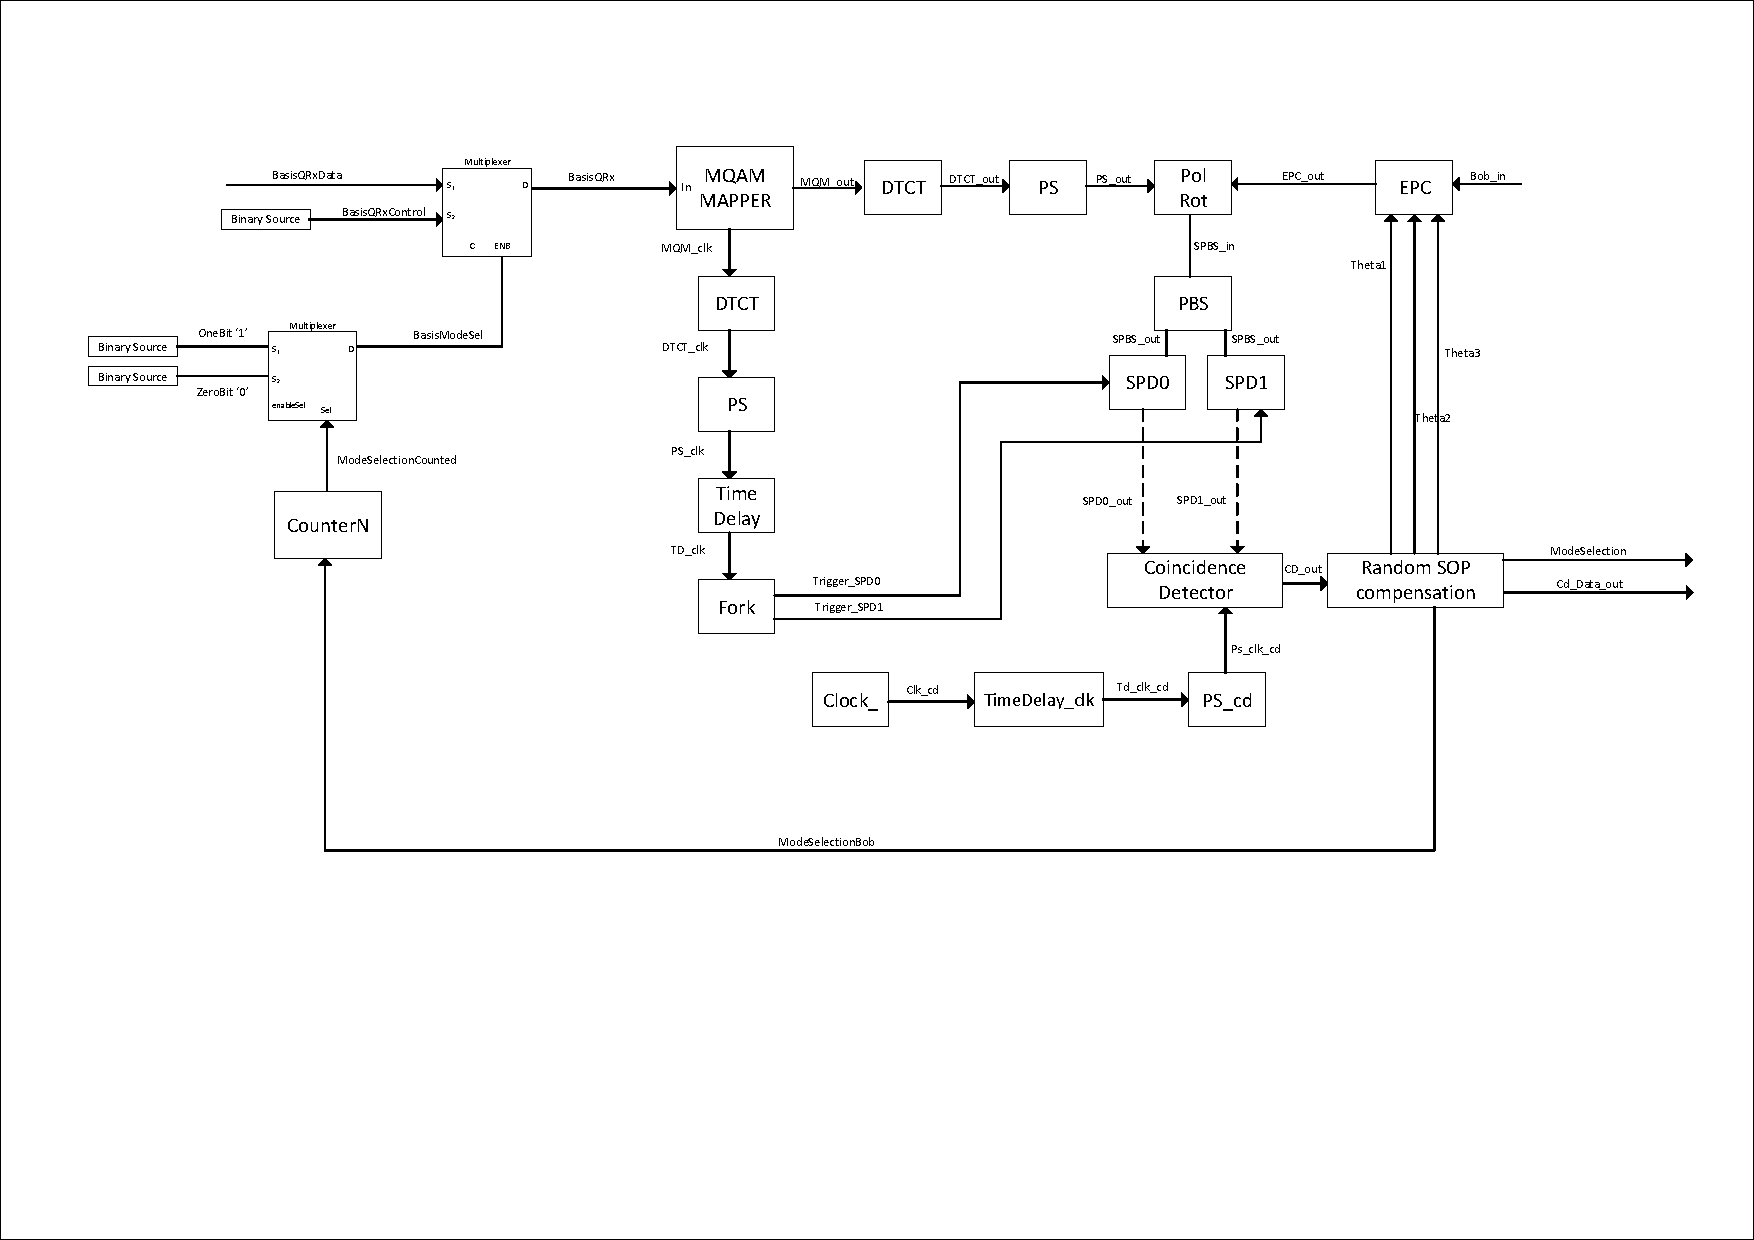
\includegraphics[clip, trim=0.5cm 6.0cm 0.5cm 2cm, width=1.0\textwidth]{./lib/BobQuantumRx/figures/BobQRx_diagram.pdf}
	\caption{Schematic of Bob Quantum Receiver}\label{bobQuantumRxDiagram}
\end{figure}

This block receives 1 input binary signal that will have the information about basis ("BobQRxBasis") to measure the single-photons that arrives from the quantum channel. This signal must comprise two possible values corresponding to two non-orthogonal basis used in the communication protocol. It also accepts a PhotonStreamXY signal corresponding to the encoded single photon that arrives from quantum channel sent by AliceQTx.

The mode selection signal that outputs this superblock will inform Alice about which mode she should selects, and so that if she should send data or control qubits.

Apart from the detection scheme, this block also comprises an active random polarization drift compensation scheme. This scheme includes a randomSopCompensation block that is responsible for all post processing tasks, including QBER estimation, and sends three feedback signals with information about the rotations to be performed by an electronic polarization controller (EPC). In this way, the random polarization drift is compensated before the single photons reach the detection scheme.


\subsection*{Input Signals}
\paragraph*{Number}: 2
\paragraph*{Type}: Binary, PhotonStreamXY.

\subsection*{Output Signals}
\paragraph*{Number}: 1
\paragraph*{Type}: Binary.

\subsection*{Examples}


\subsection*{Sugestions for future improvement}



